\chapter{Introduzione}

\subsubsection{What is an intelligent system (IS)}
\begin{center}
    \textit{a computer-based system that aims to replicate human cognitive abilities such as learning, perception, reasoning, and decision-making. }
\end{center}





\noindent By utilizing Machine Learning (ML), and other related technologies, these systems are capable of processing and analyzing data 
\hl{to perform tasks that typically require human intelligence}, make predictions, or provide insights.

\noindent Some examples of intelligent systems are:
\begin{itemize}
    \item virtual assistant like Siri and Alexa 
    \item autonomous vehicles 
    \item image recognition 
    \item fraud detection 
    \item \textit{and many others \dots}
\end{itemize}

\subsubsection{Diffusion and relevance}
In particular, ML allows us to \hl{process data at unprecedented scales}:
\begin{itemize}
    \item see patterns 
    \item detect problems earlier 
    \item allocate resources more effeciently
\end{itemize}

\newpage
\section{Major AI advancements \textcolor{blue}{[overview]}}

\subsubsection{Some recent improvements}
\begin{itemize}
    \item so-called \textbf{word embeddings} that are used as input to a Neural Network; it is 
    a set of techiniques in NLP where words are mapped to \textbf{vectors of real numbers}

    \begin{figure}[H]
        \centering
        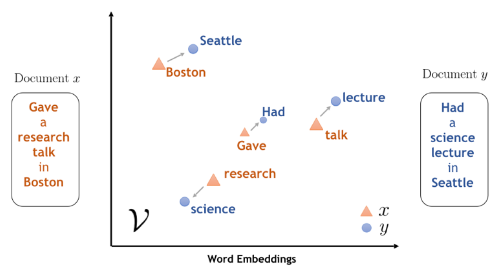
\includegraphics[width=0.6\linewidth]{01/images/word-embeddings.png}
    \end{figure}
    \item solving \textbf{analogy puzzles}
    
    \textit{Paris is to France as Tokyo is to \dots?}

    \texttt{Japan}
\end{itemize}


\subsubsection{Artificial VS Natural brain}

NN can already carry ou complex cognitive tasks, but are currently somewhere between 
the neural capacity of a bee's and a frog's brain; human brains are at least \textbf{several oreders 
of magnitude larger} than current neural networks.


\subsection{Major AI advancements in the last 2 years}
AI has made significant progress across various domains, revolutionizing 
industries and starting to create profits\dots

\subsubsection{Generative}
The introduction of GPT-4 by OpenAI has brought significant improvements in \hl{text 
generation, reasoning, and multimodal capabilities.} These models are now widely used 
in \textbf{coding assistance, creative writing, and problem-solving across various 
industries.}

\subsubsection{Coding}
AI for code generation and automation:
\begin{itemize}
    \item \hl{coding assistant} have revolutionized software development, boosting productivity 
    and reducing errors 
    \item AI-driven \hl{debugging and optimization} tools are making software development more efficient and accessible
\end{itemize}

\subsubsection{Multimodal}
AI systems have evolved to handle \hl{multiple types of inputs, including text, images, 
audio and video, simultaneously.}

\subsubsection{Diffusion}
Diffusion models for image and video generation; the quality and flexibility of 
AI-generated content is advancing.

\subsubsection{Scientific discovery}
Examples are protein structure prediction, biological research, discovering new 
compounds and accelerating innovation in chemistry.

\subsubsection{Robotics}
Real-time AI in robotics and automation, such as humanoid robot and industrial 
automation.

\subsubsection{Edge AI}
Edge AI and on-device processing: advancements in hardware allow AI models to run 
efficiently on mobile devices and edge computing platforms.

\subsubsection{AI act}
AI regulation and ethical considerations.

\subsubsection{Self-supervised and continual}
AI models are increasingly able to learn from unlabelled data and adapt to new 
tasks with minimal human intervention:
\begin{itemize}
    \item self-supervised techiniques are applied in medical imaging, such as AI models 
    detecting anomalies in X-rays without requiring extensive labeled datasets 
    \item continual learning in used in autonomous systems, such as self-driving cars, to adapt 
    to new environments without requiring complete retraining
\end{itemize}

\section{\textit{Can I use Chat-GPT?} \textcolor{darkgreen}{[tools]}}
It's a good idea to use LLM to design IS (with some warnings).

\noindent \textcolor{darkgreen}{Useful features for Intelligent Systems Design:}
\begin{itemize}
    \item ideas and brainstorming 
    \item codign assistance 
    \item data analysis and explainations
    \begin{itemize}
        \item can process large datasets and generate reports
        \item useful for creating technical documentation and explaining AI methodologies
    \end{itemize}
\end{itemize}

\noindent \textcolor{red}{Critical considerations:}
\begin{itemize}
    \item \textbf{Hallucinations:} LLMs can generate incorrect or misleading informatoin, requiring 
    careful validation
    \item \textbf{Data privacy and Security:} using LLMs for sensitive data may violate GDPR compliance
    \item \textbf{Bias in AI:} LLMs might reflect bias present in training data 
    \item \textbf{Dependency on training data:} results may be outdated

\end{itemize}

\section{Natural Interaction \textcolor{orange}{[theory]}}
Deep Learning will permit to have a natural human machine interaction; is now able (and will improve)
to \textbf{understand language, gestures, emotions, reason and interact} with humans 
in a more \textit{natural (human-like)} way.

\noindent Key modalities (for ISs):
\begin{itemize}
    \item speech-based interaction and NLP 
    \item gesture-based interaction 
    \item haptic interaction 
    \item visual and emotional recognition
\end{itemize}

\subsubsection{Limits of NLP}
Even though now has an \textbf{error rate $<$5\%}, compared to more than 10\% just a few years 
ago, it is still too high; it is suggested that naturally interacting with a computer 
will not happen until we reach errors rates of $<$1\%

\section{Biases, improvements, limitations \textcolor{orange}{[theory]}}

NN are good at learning \textbf{human biases} (systematically pattern of 
deviation from rationality in judgement).

\subsubsection{Example of a different AI bias}
\begin{itemize}
    \item suppose to have an X-ray image recognition for fractures in bones from multiple hospitals 
    \item the algorithm start to recognize which hospital generated the image 
    \item one hospital, bigger than the others, generates more bone fractures
    \item the algorithm starts to predict fractures very well \textbf{simply by recognizing 
    which hospital did the scan}, without actually looking at the bone
\end{itemize}

\section{Data-knowledge spectrum}
Where is the knowledge in the data?

\begin{figure}[H]
    \centering
    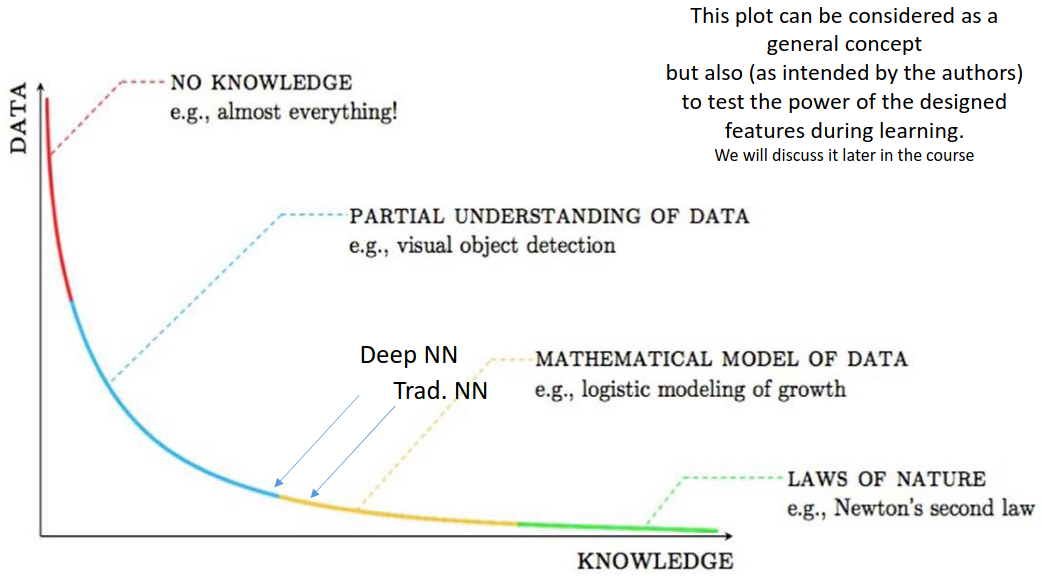
\includegraphics[width=0.8\linewidth]{01/images/dat-knowledge spectrum.png}
\end{figure}

\section{Autonomous vehicles \textcolor{red}{[use cases]}}

\begin{figure}[H]
    \centering
    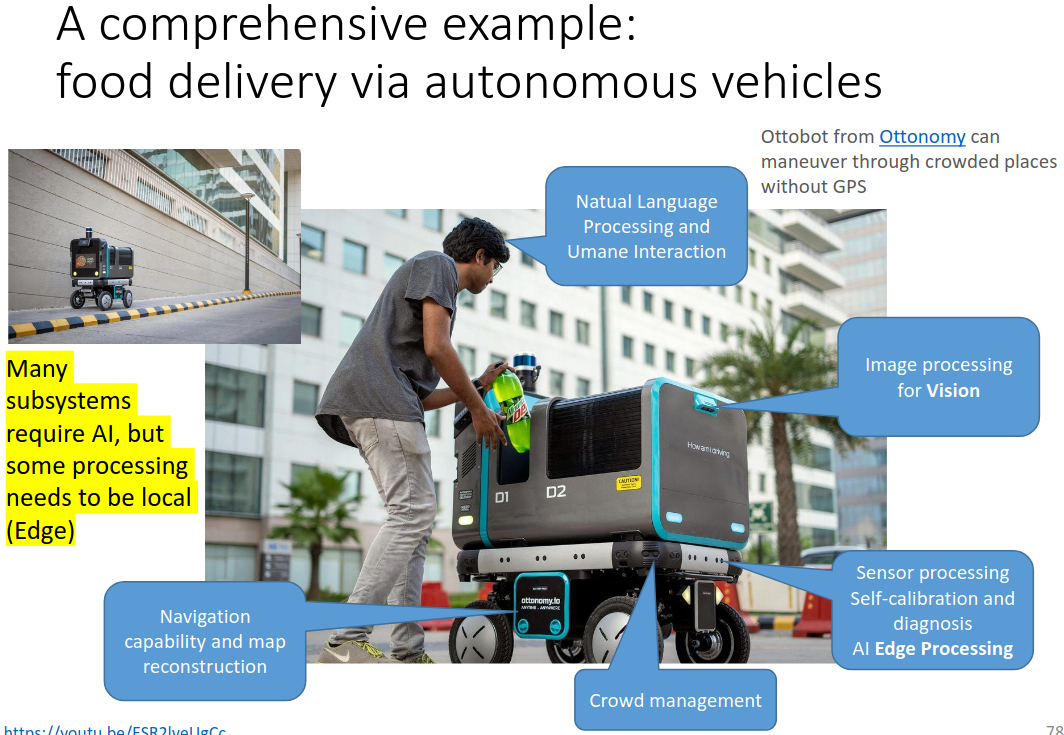
\includegraphics[width=1\linewidth]{01/images/use-case.png}
\end{figure}



